\documentclass[red]{mecanica_quantica}


\usepackage[english, portuguese]{babel}
 
\usepackage{blindtext}
\usepackage{float} 
 
\Curso{Mecânica Quântica 2017} 
\Docente{Prof. Luiz Nunes (IFSC-USP)}

\tituloAtividade{Lista 2}
\GrupoID{Grupo Z}
\Titulo{Exercícios Resolvidos}


\Autores{Krissia de Zawadzki\inseresimbolocurso{FC}, Luiz Nunes de Oliveira\inseresimbolocurso{F}} % Authors
\cursosalunos{\inseresimbolocurso{F}\textit{Bacharelado em Física}}
\cursosalunos{\inseresimbolocurso{FC}\textit{Bacharelado em Física Computacional}} 
\cursosalunos{\inseresimbolocurso{BF}\textit{Bacharelado em Ciências Físicas e Biomoleculares}} 


\dataEntrega{10 de Abril de 2017}
 
\begin{document}
 
\maketitle
\thispagestyle{fancy}
 
%\noindent
Vamos resolver abaixo alguns problemas das listas.
 
\section[]{Problema 7 - Lista 2}
 
Uma partícula no poço infinito tem a seguinte função de onda no instante inicial $t = 0$
	
	\begin{equation}
	\label{eq:Psit0}
	\Psi(x,0) = A x (a-x).
	\end{equation}


	\begin{itemize}
		\item[a)] Normalize $\Psi(x,0)$. Esboce seu gráfico. Qual estado estacionário é o mais parecido?
		Nesta base, estime o valor esperado da energia.
		\item[b)] Calcule $\valoresperado{x}$, $\valoresperado{p}$ e 
		$\valoresperado{H}$ em $t=0$. (\emph{Observação}: Desta vez você não pode calcular $\valoresperado{p}$ 
		tomando a derivada de $\valoresperado{x}$, pois $\valoresperado{x}$ é conhecido em um único instante de tempo.) 
		Como $\valoresperado{H}$ se compara à estimativa obtida em a)?
	\end{itemize} 
 
\subsection{Solução}
	
	a) \emph{Normalizando a função de onda}:
	
	Queremos
	\begin{align}
	\label{eq:normPsi}
		\int_{-\infty}^{+\infty} \, dx \,  |\Psi(x,0)|^2 = 1.
	\end{align}
	
	Assim, como $\Psi(x,0)$ está definita em $ 0 \leq x \leq a$, a constante $A$ pode ser determinada substituindo a eq. \refeq{eq:Psit0} em \refeq{eq:normPsi} e ajustando convenientemente os limites de integração.
	Segue que
	\begin{align}
	\label{eq:normPsit0}
		\int_{0}^{a} \, dx \,  |A|^2 x^2 (x-a)^2 & = 1 \nonumber \\
		%|A|^2 \, \int_{0}^{a} \, dx \, (x^4 - 2 ax^3 + a^2 x^2) & = 1 \nonumber \\ 
		A^2  \, a^5 (\frac{1}{5}- \frac{1}{2} + \frac{1}{3}) & = 1 \nonumber \\ 
		%A^2  \, \frac{a^5}{30}  & = 1 \nonumber \\ 
		A & = \sqrt{\frac{30}{a^5} }.
	\end{align}

		
	\emph{Esboçando o gráfico da função de onda:}
	
A função de onda tem a cara de uma parábola invertida que se anula para x = 0 e x = a. Assim, se compararmos com a função de onda $\psi_1(x)$ no primeiro estado estacionário (n=1), existe uma 'chance' de elas serem próximas entre si. 

\begin{minipage}{\linewidth}
      \centering
      \begin{minipage}{0.325\linewidth}
Uma forma de verificar isso é plotando as funções de onda que são soluções da parte espacial (soluções estacionárias) de $\Psi(x,t) = \psi(x) * f(t)$ no caso do poço infinito.
	Lembremos que a soluções estacionárias da função de onda da partícula no poço infinito são dadas por
		\begin{align}
		\label{eq:Psipoco}
			\psi_n(x) & = \sqrt{\frac{2}{a}} \sin{\frac{n\pi x}{a}}  \nonumber \\ 
			& n = 1, 2, ...,
		\end{align}
		com energias
		\begin{align}
		\label{eq:energiapoco}
			E_n & = \frac{\hbar^2 \pi^2}{2m a^2} n^2 \nonumber \\
			n = 1, 2, ...
		\end{align}
	


      \end{minipage}
      \hspace{0.05\linewidth}
      \begin{minipage}{0.6\linewidth}
 
       	\begin{figure}[H]
	\begin{center}
		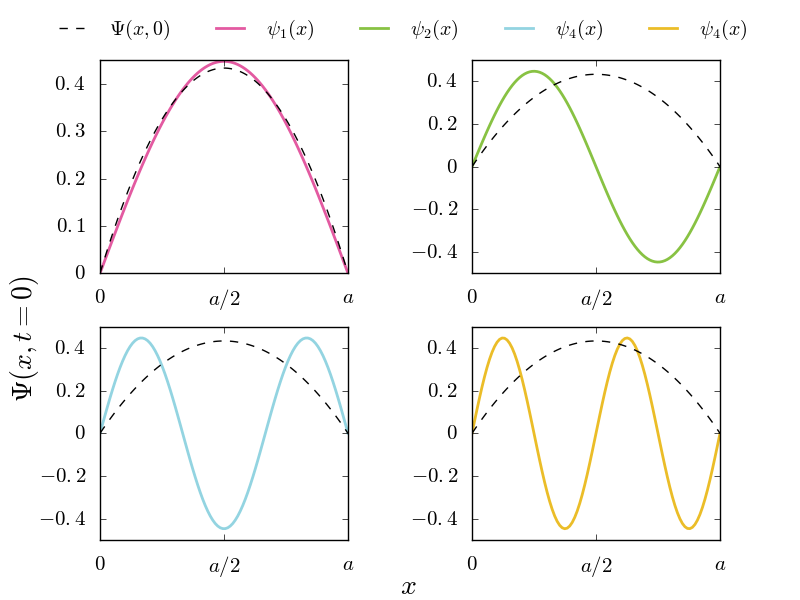
\includegraphics[scale=0.5]{../2lista_prob7}
		\caption{Estados estacionários do poço infinito -- eq. \refeq{eq:Psipoco}  -- (linhas cheias coloridas) e função de onda no instante $t=0$ -- eq. \refeq{eq:Psit0}. }
		\label{fig:funcaodeonda}
	\end{center}
	\end{figure}    


      \end{minipage}
  \end{minipage}

 


Da figura \refig{fig:funcaodeonda} podemos notas que $\psi_1(x)$ é muito próxima à função de onda $\Psi(x,t=0)$ na eq. \refeq{eq:Psit0}. Isso nos possibilita estimar qualquer observável associado a este sistema nesse estado usando os resultados que teríamos para $\psi_1(x)$ ! 

Desse modo, o valor esperado para a energia pode ser tomado como, aproximadamente,
	\begin{equation}
	\label{eq:Eapprox}
	\valoresperado{E} \approx E_1 = \frac{\hbar^2 \pi^2}{2m a^2}.
	\end{equation}

	
	b) \emph{Calculando valores esperados}
	
	Para calcular o valor esperado $\valoresperado{O}$ associado a qualquer observável $\operador{O}$ associado à partícula quando esta é descrita por uma função de onda $\Psi(x,t)$, 
	fazemos
	
	\begin{equation}
	\label{eq:calcvaloresperado}
		\valoresperado{O}(t) = \int_{-\infty}^{+\infty} \, dx \,  \Psi^*(x,t) \operador{O} \,  \Psi(x,t)
		.
	\end{equation}


	Para o caso da posição inicial, temos
	\begin{align}
	\label{eq:x0esp}
		\valoresperado{x} & = \int_{0}^{a} \, dx \,  \Psi^*(x,0) x \,  \Psi(x,0) \nonumber \\
		& = \int_{0}^{a} \, dx \,  A^2 x^3 (x-a)^2 \nonumber \\
		& = A^2 \frac{a^6}{60} \nonumber \\
		& = \frac{a}{2},
	\end{align}
	ou seja, a posição 'média' em que encontramos a partícula é na metade da caixa!
	Se voltarmos na nossa figura \refig{fig:funcaodeonda}, notamos que a densidade de probabilidade é máxima quando $x=a/2$, seja com a função de onda dada pela eq. \refeq{eq:Psit0} ou sua parente próxima \refeq{eq:Psipoco} com $n=1$.
	
	Para o valor esperado do momento $\valoresperado{p}$, precisamos de uma observação. Em Mecânica Quântica, grandezas físicas estão associadas a operadores que, ao atuarem na função de onda, a modificam. O momento está associado operador $\operador p$ que, para sistemas unidimensionais, é definido por 
	\begin{equation}
		\label{eq:operadorp}
		\operador{p} = -i\hbar \frac{\partial}{\partial x}.
	 \end{equation} 
	 
	 Assim, o valor esperado $\valoresperado{p}$ é calculado como segue
	 \begin{align}
	 \label{eq:p0esp}
	 	\valoresperado{p} & = \int_{0}^{a} \, dx \,  \Psi^*(x,0) \, -i\hbar \frac{\partial}{\partial x} \,  \Psi(x,0) \nonumber \\
	 	& = -i\hbar \int_{0}^{a} \, dx \, A^2 x(a-x)(a-2x) \nonumber \\
	 	& = 0.
	 \end{align}
	 
	 Note que esta solução faz sentido, pois significa que, em média, a partícula está viajando com momentos $p > 0$ e $p < 0$, que são equivalentes.
	 
	 Finalmente, vamos calcular o valor esperado para $\valoresperado{H}$. Recordemos o operador quântico $\hat{H}$ está associado às energias do sistema. Ele é dado por
	 \begin{equation}
	 	\label{eq:operadorH}
	 	H = -\frac{\hbar^2}{2m} \frac{\partial^2}{\partial x^2}.
	 \end{equation}
	 
	 Logo, a quantidade que nos interessa é calculada como
	 \begin{align}
	 \label{eq:E0esp}
	 	\valoresperado{H} & = \int_{0}^{a} \, dx \,  \Psi^*(x,0) \, -\frac{\hbar^2}{2m} \frac{\partial^2}{\partial x^2} \,  \Psi(x,0) \nonumber \\
	 	& =-\frac{\hbar^2}{2m} \int_{0}^{a} \, dx \, A^2 x(a-x)(-2) \nonumber \\
	 	& = \frac{\hbar^2}{2m} A^2 \frac{a^3}{3} \nonumber \\
	 	& = \frac{10 \hbar^2}{2m a^2}.
	 \end{align}	 
	 
	 Voltando à nossa estimativa para a energia, eq. \refeq{eq:Eapprox}, e lembrando que $\pi^2 \approx |\vec{g}|^2 \approx 10$ \footnote{Sim! Pelo menos, foi o que eu medi no laboratório de Física 1 em 2008 ...}, concluímos que nossa aproximação foi muito boa.
	 
\end{document}
